% Insert early so the single-column float can occupy the first page's
% right-column top, alongside the abstract, using standard ACM float placement.
\noindent\textbf{Relevance Statement.}
This work is relevant to the Web Infrastructure and Agentic Systems track. Web agents use reusable task instructions, or skills, across requests and services. We examine when skill-state transfer weakens despite the original run's continued skill dependence, and how attention caches partly restore transfer. These findings inform the evaluation of skill reuse and context management for Web agents.


\begin{figure}[t]
\centering
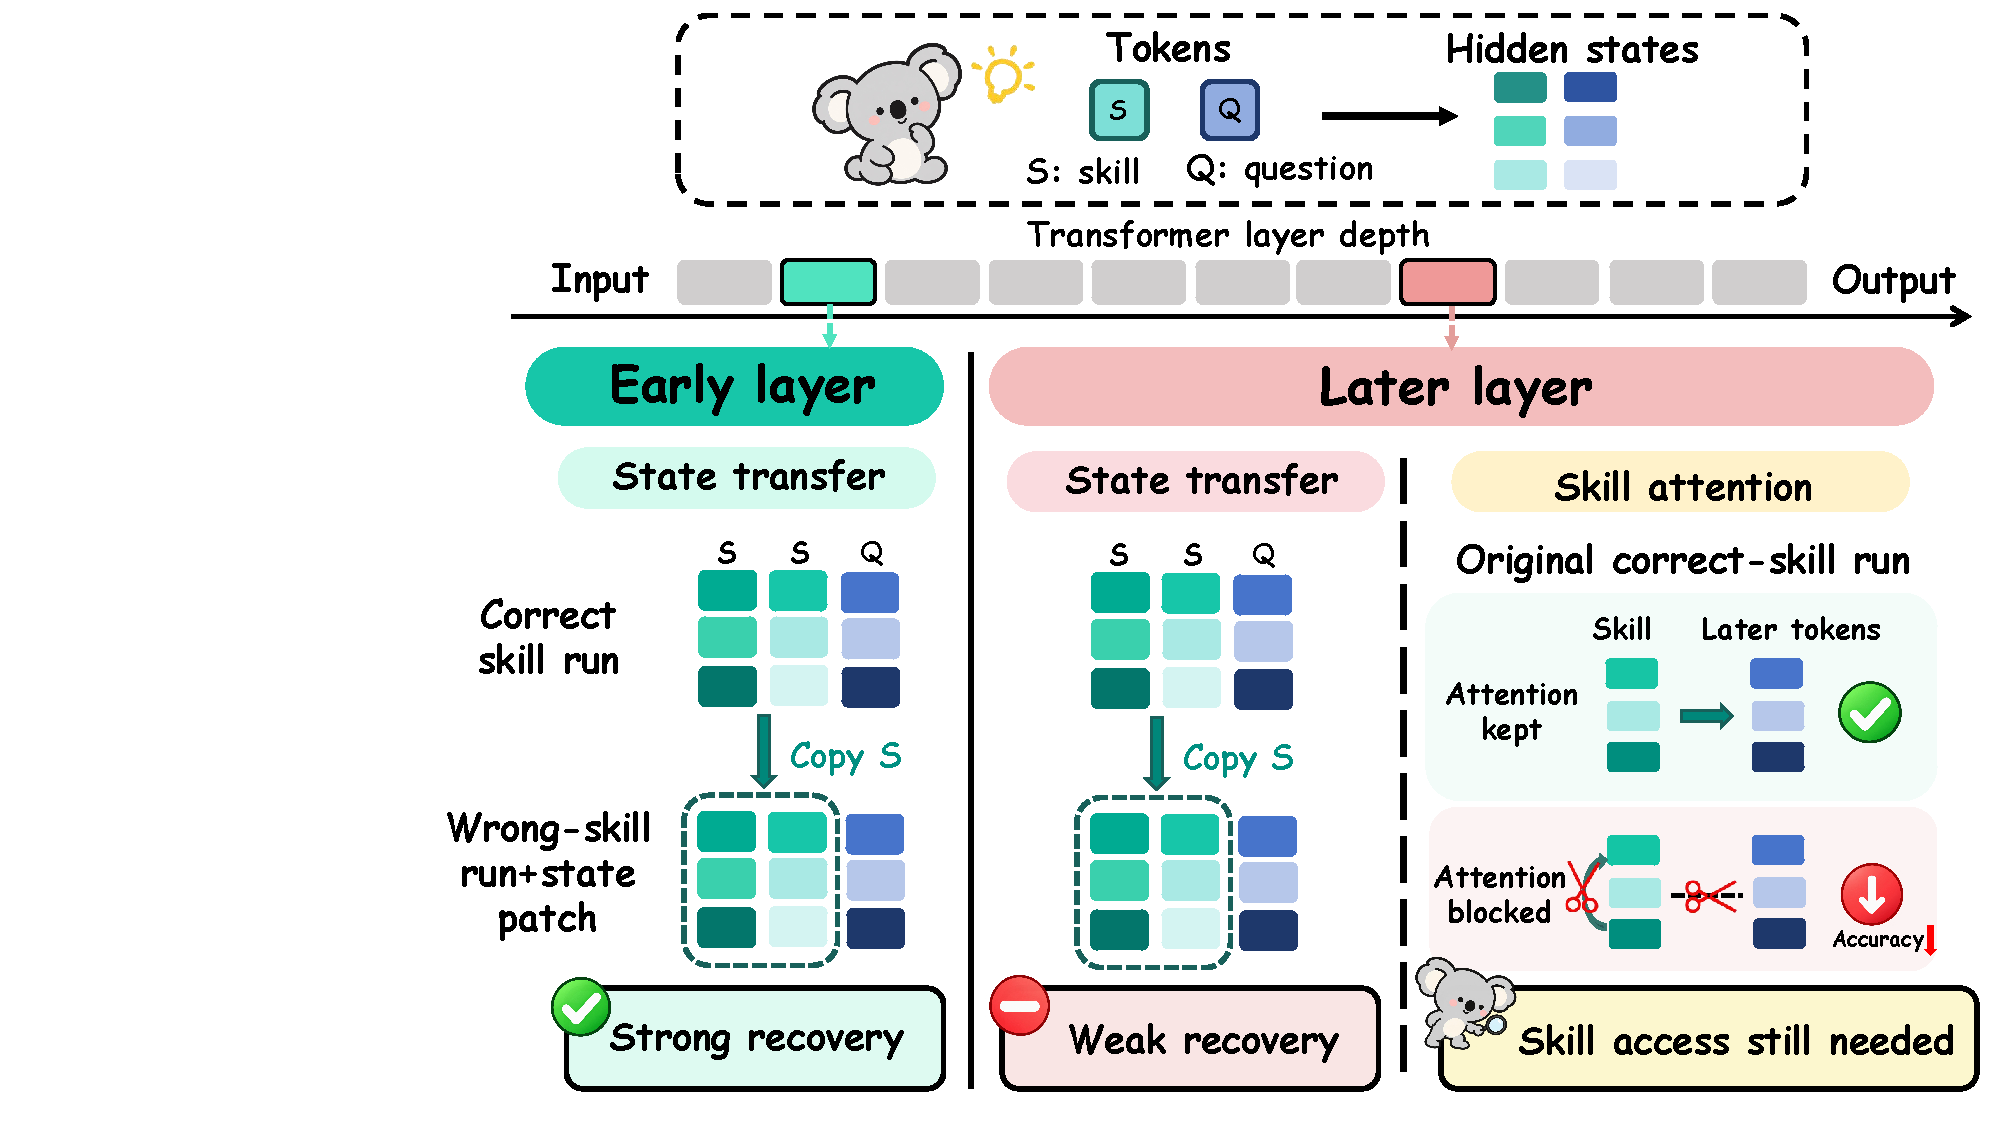
\includegraphics[width=\columnwidth]{fig-teaser.pdf}
\caption{Weak transfer and continued skill use at the same later depth.
Copying skill-position states from a correct-skill run into an unrelated-skill
run gives strong early recovery (left) and weak late recovery (middle).
At that same later depth, the original run still needs skill access:
retaining access preserves performance, while cutting it reduces accuracy
(right). S and Q label skill and question tokens.
Figure~\ref{fig:transferreading} gives the measured depth profiles.}
\Description{A schematic follows transformer depth from input to output.
At an early layer, replacing skill-position hidden states yields strong
recovery. At a later layer the same type of replacement yields weak recovery.
In the original correct-skill run at that later layer, retaining skill access
preserves performance while cutting access reduces accuracy. Green blocks
represent skill tokens and blue blocks question tokens.}
\label{fig:teaser}
\end{figure}

\section{Introduction}
\label{sec:intro}

Language models can perform new tasks by following instructions provided
in context. Reusable skills organize such instructions into descriptions
of how to carry out a task \citep{zhang2025agentskills}. Web agents use
skills and workflows to guide actions across requests and services
\citep{wang2024awm,wang2026webxskill}. A calculator skill, for example,
specifies a formula, input conventions and steps for applying them to a
new question. As a model processes a skill, it forms hidden states,
internal vectors associated with the instruction tokens. Reusing these
states could allow one execution to supply task-relevant information to
another without changing the model's weights.

Prior work transfers task information through internal vectors derived
from demonstrations or attention outputs
\citep{hendel2023taskvectors,todd2024functionvectors}. Layer-wise
interventions separately examine where state replacement loses its
effect and where attention to context becomes unnecessary
\citep{onset2025instruction,sia2024incontexttranslation}. Restoring
performance by copying states and disrupting it by blocking attention,
however, measure different effects \citep{heimersheim2024patching}.
A failed transfer does not establish that the original execution no
longer needs the skill. We ask: \emph{Can skill-state transfer weaken with
depth while the original execution remains dependent on the skill?}

We study this question through controlled question answering with skill
selection held fixed. For the same question, we compare a correct-skill
run with a run using length-matched text from an unrelated skill.
At each layer, the transfer test copies the correct-skill run's hidden
states at skill positions into the unrelated-skill run. Separately, the dependence test blocks
attention to the skill in the correct-skill run from that layer onward.
The tests use common questions within each model and task setting.
Content, position and cross-question controls assess whether early
transfer carries skill-relevant information.

Hidden-state copying does not directly replace the key/value (KV) caches
that attention uses to retain information from processed tokens.
We extend transfer by copying skill-position caches alongside hidden
states and test whether the recovered execution still needs skill
reading in later layers. Cache-only controls replace skill-position
caches at every layer.

Across four models and two benchmarks, all eight comparisons show that
transfer weakens at later layers while the original run remains strongly
dependent on the skill (Figure~\ref{fig:teaser}).

At layer $16$, joint state and cache replacement improves accuracy over states alone by $6.8$
to $43.4$ percentage points, and blocking subsequent skill reading
reduces the recovered accuracy in every setting. Copying only
skill-position caches at every layer still falls short of correct-skill
accuracy. Copying caches for all processed prompt tokens reproduces the
correct-skill run's generated sequence. Recomputing the later prompt
with correct-skill caches also brings accuracy close to that of the
correct-skill run.

Our contributions are summarized as follows:
\begin{itemize}
\item \textbf{Skill dependence persists as state transfer weakens.}
Across all eight settings, transfer weakens at later layers while the
original run remains dependent on the skill.
\item \textbf{Skill caches improve state transfer.}
Adding skill-position KV at layer $16$ improves accuracy in all eight
settings. The recovered run still depends on skill reading.
\item \textbf{Skill caches alone do not restore correct-skill accuracy.}
With all skill-position caches restored, copying the remaining prefix
caches or recomputing the later prompt improves recovery.
\end{itemize}
